\tinysidebar{\debug{exercises/{exercises0/question.tex}}}
I'm going to make some changes to the doubly linked list.
Here's a doubly linked list (without sentinel nodes):

\input{stdout41.tex}

The usual delete tail will result in this:

\begin{center}
\begin{tikzpicture}

\fill[white] (19.0, -0.6) circle (0.3);
\node [line width=0.03cm,black,minimum size=0.57cm,draw,circle] at (19.0,-0.6)(A){};\draw (19.0, -0.6) node[color=black] {\texttt{20}};
\fill[white] (16.0, -1.0) circle (0.3);
\node [line width=0.03cm,black,minimum size=0.57cm,draw,circle] at (16.0,-1.0)(a){};\draw (16.0, -1.0) node[color=black] {\texttt{10}};
\fill[white] (10.0, -2.0) circle (0.3);
\node [line width=0.03cm,black,minimum size=0.57cm,draw,circle] at (10.0,-2.0)(b){};\draw (10.0, -2.0) node[color=black] {\texttt{0}};
\fill[white] (11.0, -4.0) circle (0.3);
\node [line width=0.03cm,black,minimum size=0.57cm,draw,circle] at (11.0,-4.0)(d){};\draw (11.0, -4.0) node[color=black] {\texttt{18}};
\fill[white] (8.0, -3.0) circle (0.3);
\node [line width=0.03cm,black,minimum size=0.57cm,draw,circle] at (8.0,-3.0)(e){};\draw (8.0, -3.0) node[color=black] {\texttt{-2}};
\fill[white] (7.0, -4.0) circle (0.3);
\node [line width=0.03cm,black,minimum size=0.57cm,draw,circle] at (7.0,-4.0)(k){};\draw (7.0, -4.0) node[color=black] {\texttt{-3}};
\fill[white] (9.0, -4.0) circle (0.3);
\node [line width=0.03cm,black,minimum size=0.57cm,draw,circle] at (9.0,-4.0)(l){};\draw (9.0, -4.0) node[color=black] {\texttt{-1}};
\fill[white] (15.0, -4.0) circle (0.3);
\node [line width=0.03cm,black,minimum size=0.57cm,draw,circle] at (15.0,-4.0)(h){};\draw (15.0, -4.0) node[color=black] {\texttt{8}};
\fill[white] (14.0, -5.0) circle (0.3);
\node [line width=0.03cm,black,minimum size=0.57cm,draw,circle] at (14.0,-5.0)(m){};\draw (14.0, -5.0) node[color=black] {\texttt{6}};
\fill[white] (13.0, -3.0) circle (0.3);
\node [line width=0.03cm,black,minimum size=0.57cm,draw,circle] at (13.0,-3.0)(f){};\draw (13.0, -3.0) node[color=black] {\texttt{5}};
\fill[white] (13.0, -6.0) circle (0.3);
\node [line width=0.03cm,black,minimum size=0.57cm,draw,circle] at (13.0,-6.0)(n){};\draw (13.0, -6.0) node[color=black] {\texttt{4}};
\fill[white] (15.0, -6.0) circle (0.3);
\node [line width=0.03cm,black,minimum size=0.57cm,draw,circle] at (15.0,-6.0)(o){};\draw (15.0, -6.0) node[color=black] {\texttt{7}};
\fill[white] (18.0, -2.0) circle (0.3);
\node [line width=0.03cm,black,minimum size=0.57cm,draw,circle] at (18.0,-2.0)(p){};\draw (18.0, -2.0) node[color=black] {\texttt{15}};\draw[line width=0.03cm,black,->,>=triangle 60] (A) to  (a);
\draw[line width=0.03cm,black,->,>=triangle 60] (a) to  (p);
\draw[line width=0.03cm,black,->,>=triangle 60] (a) to  (b);
\draw[line width=0.03cm,black,->,>=triangle 60] (b) to  (e);
\draw[line width=0.03cm,black,->,>=triangle 60] (b) to  (f);
\draw[line width=0.03cm,black,->,>=triangle 60] (f) to  (d);
\draw[line width=0.03cm,black,->,>=triangle 60] (f) to  (h);
\draw[line width=0.03cm,black,->,>=triangle 60] (e) to  (k);
\draw[line width=0.03cm,black,->,>=triangle 60] (e) to  (l);
\draw[line width=0.03cm,black,->,>=triangle 60] (h) to  (m);
\draw[line width=0.03cm,black,->,>=triangle 60] (m) to  (n);
\draw[line width=0.03cm,black,->,>=triangle 60] (m) to  (o);
\end{tikzpicture}

\end{center}



Write a doubly linked list class that does this instead:

from latextool_basic import *
print(automata(layout="""
A  B

C  D
""",
edges="A,$a$,B|A,$b$,C|B,$a$,D|B,$b$,C|C,$b$,A|C,$a$,D|D,$a$,B|D,$b$,A",
A='initial|label=$q_0$',
B='accept|label=$q_1$',
C='label=$q_2$',
D='accept|label=$q_3$', xscale=1.3,
))


When I insert 8 as tail, I don't have to allocate memory. I just use the node
with 5, but I replace the 5 with 8:

\begin{center}
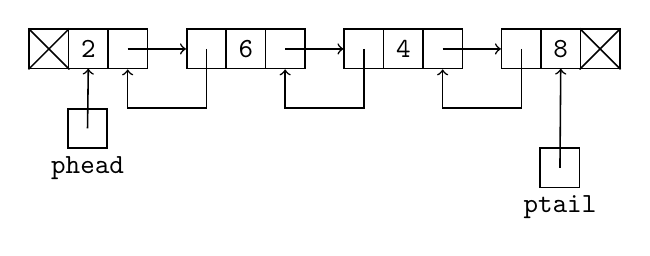
\begin{tikzpicture}

\draw (0.25, 0.25)
  node[draw, line width=0.02cm, , color=black,
       rounded corners=0cm, inner sep=0cm] {

\begin{minipage}[t][0.5cm]{0.5cm}
\mbox{}

\end{minipage}

};\draw (0.25, 0.25) node[color=black] {{\texttt{}}};
\draw (0.75, 0.25)
  node[draw, line width=0.02cm, , color=black,
       rounded corners=0cm, inner sep=0cm] {

\begin{minipage}[t][0.5cm]{0.5cm}
\mbox{}

\end{minipage}

};\draw (0.75, 0.25) node[color=black] {{\texttt{2}}};
\draw (1.25, 0.25)
  node[draw, line width=0.02cm, , color=black,
       rounded corners=0cm, inner sep=0cm] {

\begin{minipage}[t][0.5cm]{0.5cm}
\mbox{}

\end{minipage}

};\draw (1.25, 0.25) node[color=black] {{\texttt{}}};
\draw (2.25, 0.25)
  node[draw, line width=0.02cm, , color=black,
       rounded corners=0cm, inner sep=0cm] {

\begin{minipage}[t][0.5cm]{0.5cm}
\mbox{}

\end{minipage}

};\draw (2.25, 0.25) node[color=black] {{\texttt{}}};
\draw (2.75, 0.25)
  node[draw, line width=0.02cm, , color=black,
       rounded corners=0cm, inner sep=0cm] {

\begin{minipage}[t][0.5cm]{0.5cm}
\mbox{}

\end{minipage}

};\draw (2.75, 0.25) node[color=black] {{\texttt{6}}};
\draw (3.25, 0.25)
  node[draw, line width=0.02cm, , color=black,
       rounded corners=0cm, inner sep=0cm] {

\begin{minipage}[t][0.5cm]{0.5cm}
\mbox{}

\end{minipage}

};\draw (3.25, 0.25) node[color=black] {{\texttt{}}};
\draw (4.25, 0.25)
  node[draw, line width=0.02cm, , color=black,
       rounded corners=0cm, inner sep=0cm] {

\begin{minipage}[t][0.5cm]{0.5cm}
\mbox{}

\end{minipage}

};\draw (4.25, 0.25) node[color=black] {{\texttt{}}};
\draw (4.75, 0.25)
  node[draw, line width=0.02cm, , color=black,
       rounded corners=0cm, inner sep=0cm] {

\begin{minipage}[t][0.5cm]{0.5cm}
\mbox{}

\end{minipage}

};\draw (4.75, 0.25) node[color=black] {{\texttt{4}}};
\draw (5.25, 0.25)
  node[draw, line width=0.02cm, , color=black,
       rounded corners=0cm, inner sep=0cm] {

\begin{minipage}[t][0.5cm]{0.5cm}
\mbox{}

\end{minipage}

};\draw (5.25, 0.25) node[color=black] {{\texttt{}}};
\draw (6.25, 0.25)
  node[draw, line width=0.02cm, , color=black,
       rounded corners=0cm, inner sep=0cm] {

\begin{minipage}[t][0.5cm]{0.5cm}
\mbox{}

\end{minipage}

};\draw (6.25, 0.25) node[color=black] {{\texttt{}}};
\draw (6.75, 0.25)
  node[draw, line width=0.02cm, , color=black,
       rounded corners=0cm, inner sep=0cm] {

\begin{minipage}[t][0.5cm]{0.5cm}
\mbox{}

\end{minipage}

};\draw (6.75, 0.25) node[color=black] {{\texttt{8}}};
\draw (7.25, 0.25)
  node[draw, line width=0.02cm, , color=black,
       rounded corners=0cm, inner sep=0cm] {

\begin{minipage}[t][0.5cm]{0.5cm}
\mbox{}

\end{minipage}

};\draw (7.25, 0.25) node[color=black] {{\texttt{}}};\draw[line width=0.02cm,black,->] (1.25,0.25) to  (1.99,0.25);
\draw[line width=0.02cm,black,->] (3.25,0.25) to  (3.99,0.25);
\draw[line width=0.02cm,black,->] (2.25,0.25) to  (2.25,-0.5) to  (1.25,-0.5) to  (1.25,-0.01);
\draw[line width=0.02cm,black,->] (5.25,0.25) to  (5.99,0.25);
\draw[line width=0.02cm,black,->] (4.25,0.25) to  (4.25,-0.5) to  (3.25,-0.5) to  (3.25,-0.01);
\draw[line width=0.02cm,black,->] (6.25,0.25) to  (6.25,-0.5) to  (5.25,-0.5) to  (5.25,-0.01);
\draw[line width=0.02cm,black] (-0.01,0.51) to  (0.51,-0.01);
\draw[line width=0.02cm,black] (0.51,0.51) to  (-0.01,-0.01);
\draw[line width=0.02cm,black] (6.99,0.51) to  (7.51,-0.01);
\draw[line width=0.02cm,black] (7.51,0.51) to  (6.99,-0.01);

\draw (0.74, -0.76)
  node[draw, line width=0.02cm, , color=black,
       rounded corners=0cm, inner sep=0cm] {

\begin{minipage}[t][0.5cm]{0.5cm}
\mbox{}

\end{minipage}

};\draw (0.74, -0.76) node[color=black] {{\texttt{}}};
\draw (0.74, -1.26)
  node[draw, line width=0.02cm, , color=white,
       rounded corners=0cm, inner sep=0cm] {

\begin{minipage}[t][0.1cm]{0.1cm}
\mbox{}

\end{minipage}

};\draw (0.74, -1.26) node[color=black] {{\texttt{phead}}};\draw[line width=0.02cm,black,->] (0.74,-0.76) to  (0.75,0);

\draw (6.74, -1.26)
  node[draw, line width=0.02cm, , color=black,
       rounded corners=0cm, inner sep=0cm] {

\begin{minipage}[t][0.5cm]{0.5cm}
\mbox{}

\end{minipage}

};\draw (6.74, -1.26) node[color=black] {{\texttt{}}};
\draw (6.74, -1.76)
  node[draw, line width=0.02cm, , color=white,
       rounded corners=0cm, inner sep=0cm] {

\begin{minipage}[t][0.1cm]{0.1cm}
\mbox{}

\end{minipage}

};\draw (6.74, -1.76) node[color=black] {{\texttt{ptail}}};\draw[line width=0.02cm,black,->] (6.74,-1.26) to  (6.75,0);
\end{tikzpicture}

\end{center}



In other words, we delay the deallocation of head and tail nodes.
We can think of the used but not deallocated nodes as extra nodes
waiting to be reused.
When we do want to release the memory, we call the
\verb!shrink_to_fit()!.
Likewise, the same tbing happens at the end.

Next, add sentinel nodes:

\begin{center}
\begin{tikzpicture}

\fill[white] (19.0, -0.6) circle (0.3);
\node [line width=0.03cm,black,minimum size=0.57cm,draw,circle] at (19.0,-0.6)(A){};\draw (19.0, -0.6) node[color=black] {\texttt{20}};
\fill[white] (16.0, -1.0) circle (0.3);
\node [line width=0.03cm,black,minimum size=0.57cm,draw,circle] at (16.0,-1.0)(a){};\draw (16.0, -1.0) node[color=black] {\texttt{10}};\draw[line width=0.1cm,black] (15.8,-1.2) to  (16.2,-0.8);

\fill[white] (16.0, -2.0) circle (0.3);
\node [line width=0.03cm,white,minimum size=0.57cm,draw,circle] at (16.0,-2.0)(aa){};\draw (16.0, -2.0) node[color=black] {\texttt{0}};\draw[line width=0.05cm,black,->,>=triangle 60] (aa) to  (a);

\fill[white] (10.0, -2.0) circle (0.3);
\node [line width=0.03cm,black,,dashed,minimum size=0.57cm,draw,circle] at (10.0,-2.0)(b){};\draw (10.0, -2.0) node[color=black] {\texttt{0}};
\fill[white] (8.0, -3.0) circle (0.3);
\node [line width=0.03cm,black,minimum size=0.57cm,draw,circle] at (8.0,-3.0)(e){};\draw (8.0, -3.0) node[color=black] {\texttt{-2}};
\fill[white] (7.0, -4.0) circle (0.3);
\node [line width=0.03cm,black,minimum size=0.57cm,draw,circle] at (7.0,-4.0)(k){};\draw (7.0, -4.0) node[color=black] {\texttt{-3}};
\fill[white] (9.0, -4.0) circle (0.3);
\node [line width=0.03cm,black,minimum size=0.57cm,draw,circle] at (9.0,-4.0)(l){};\draw (9.0, -4.0) node[color=black] {\texttt{-1}};
\fill[white] (18.0, -2.0) circle (0.3);
\node [line width=0.03cm,black,minimum size=0.57cm,draw,circle] at (18.0,-2.0)(p){};\draw (18.0, -2.0) node[color=black] {\texttt{15}};\draw[line width=0.03cm,black,->,>=triangle 60] (a) to  (e);
\draw[line width=0.03cm,black,->,>=triangle 60] (A) to  (a);
\draw[line width=0.03cm,black,->,>=triangle 60] (a) to  (p);
\draw[line width=0.03cm,black,->,>=triangle 60] (e) to  (k);
\draw[line width=0.03cm,black,->,>=triangle 60] (e) to  (l);
\draw[line width=0.03cm,black,->,>=triangle 60,dashed] (a) to  (b);
\draw[line width=0.03cm,black,->,>=triangle 60,dashed] (b) to  (e);
\end{tikzpicture}

\end{center}



Note that I'm renaming \texttt{phead} to 
\texttt{pheadsentinel}
and
\texttt{ptail}
to
\texttt{ptailsentinel}
(The \texttt{?} denotes integer values we don't care about.)
And if I delete the tail, the above becomes


\begin{center}

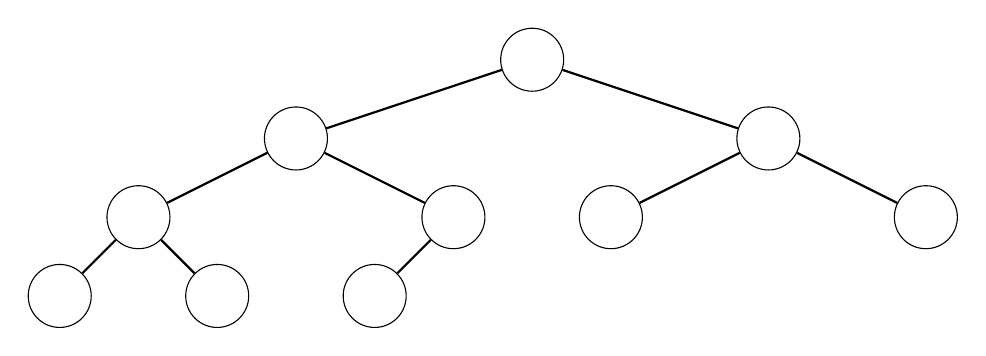
\begin{tikzpicture}
\node at (6,-1) [circle,draw,minimum size=8mm] (A) {};
\node at (3,-2) [circle,draw,minimum size=8mm] (B) {};
\node at (9,-2) [circle,draw,minimum size=8mm] (C) {};
\node at (1,-3) [circle,draw,minimum size=8mm] (D) {};
\node at (5,-3) [circle,draw,minimum size=8mm] (E) {};
\node at (7,-3) [circle,draw,minimum size=8mm] (F) {};
\node at (11,-3) [circle,draw,minimum size=8mm] (G) {};
\node at (0,-4) [circle,draw,minimum size=8mm] (H) {};
\node at (2,-4) [circle,draw,minimum size=8mm] (I) {};
\node at (4,-4) [circle,draw,minimum size=8mm] (J) {};
\draw [-,thick] (A) -- (B);
\draw [-,thick] (A) -- (C);
\draw [-,thick] (B) -- (D);
\draw [-,thick] (B) -- (E);
\draw [-,thick] (C) -- (G);
\draw [-,thick] (C) -- (F);
\draw [-,thick] (D) -- (H);
\draw [-,thick] (D) -- (I);
\draw [-,thick] (E) -- (J);

;
\end{tikzpicture}
    
\end{center}



At this point, the size of the linked list is (of course) 3
and the capacity is 4.

Of course the linked list starts off as an empty list
that looks like this (there are two sentinel nodes)

\begin{center}
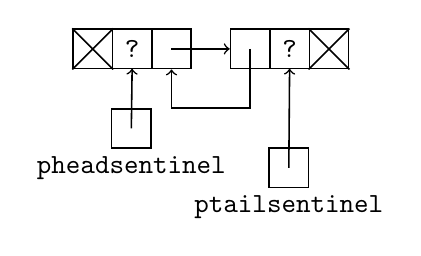
\begin{tikzpicture}

\draw (0.25, 0.25)
  node[draw, line width=0.02cm, , color=black,
       rounded corners=0cm, inner sep=0cm] {

\begin{minipage}[t][0.5cm]{0.5cm}
\mbox{}

\end{minipage}

};\draw (0.25, 0.25) node[color=black] {{\texttt{}}};
\draw (0.75, 0.25)
  node[draw, line width=0.02cm, , color=black,
       rounded corners=0cm, inner sep=0cm] {

\begin{minipage}[t][0.5cm]{0.5cm}
\mbox{}

\end{minipage}

};\draw (0.75, 0.25) node[color=black] {{\texttt{?}}};
\draw (1.25, 0.25)
  node[draw, line width=0.02cm, , color=black,
       rounded corners=0cm, inner sep=0cm] {

\begin{minipage}[t][0.5cm]{0.5cm}
\mbox{}

\end{minipage}

};\draw (1.25, 0.25) node[color=black] {{\texttt{}}};
\draw (2.25, 0.25)
  node[draw, line width=0.02cm, , color=black,
       rounded corners=0cm, inner sep=0cm] {

\begin{minipage}[t][0.5cm]{0.5cm}
\mbox{}

\end{minipage}

};\draw (2.25, 0.25) node[color=black] {{\texttt{}}};
\draw (2.75, 0.25)
  node[draw, line width=0.02cm, , color=black,
       rounded corners=0cm, inner sep=0cm] {

\begin{minipage}[t][0.5cm]{0.5cm}
\mbox{}

\end{minipage}

};\draw (2.75, 0.25) node[color=black] {{\texttt{?}}};
\draw (3.25, 0.25)
  node[draw, line width=0.02cm, , color=black,
       rounded corners=0cm, inner sep=0cm] {

\begin{minipage}[t][0.5cm]{0.5cm}
\mbox{}

\end{minipage}

};\draw (3.25, 0.25) node[color=black] {{\texttt{}}};\draw[line width=0.02cm,black,->] (1.25,0.25) to  (1.99,0.25);
\draw[line width=0.02cm,black,->] (2.25,0.25) to  (2.25,-0.5) to  (1.25,-0.5) to  (1.25,-0.01);
\draw[line width=0.02cm,black] (-0.01,0.51) to  (0.51,-0.01);
\draw[line width=0.02cm,black] (0.51,0.51) to  (-0.01,-0.01);
\draw[line width=0.02cm,black] (2.99,0.51) to  (3.51,-0.01);
\draw[line width=0.02cm,black] (3.51,0.51) to  (2.99,-0.01);

\draw (0.74, -0.76)
  node[draw, line width=0.02cm, , color=black,
       rounded corners=0cm, inner sep=0cm] {

\begin{minipage}[t][0.5cm]{0.5cm}
\mbox{}

\end{minipage}

};\draw (0.74, -0.76) node[color=black] {{\texttt{}}};
\draw (0.74, -1.26)
  node[draw, line width=0.02cm, , color=white,
       rounded corners=0cm, inner sep=0cm] {

\begin{minipage}[t][0.1cm]{0.1cm}
\mbox{}

\end{minipage}

};\draw (0.74, -1.26) node[color=black] {{\texttt{pheadsentinel}}};\draw[line width=0.02cm,black,->] (0.74,-0.76) to  (0.75,0);

\draw (2.74, -1.26)
  node[draw, line width=0.02cm, , color=black,
       rounded corners=0cm, inner sep=0cm] {

\begin{minipage}[t][0.5cm]{0.5cm}
\mbox{}

\end{minipage}

};\draw (2.74, -1.26) node[color=black] {{\texttt{}}};
\draw (2.74, -1.76)
  node[draw, line width=0.02cm, , color=white,
       rounded corners=0cm, inner sep=0cm] {

\begin{minipage}[t][0.1cm]{0.1cm}
\mbox{}

\end{minipage}

};\draw (2.74, -1.76) node[color=black] {{\texttt{ptailsentinel}}};\draw[line width=0.02cm,black,->] (2.74,-1.26) to  (2.75,0);
\end{tikzpicture}

\end{center}



Objects of this type of linked list have
\texttt{size()} and \texttt{capacity()}
that returns the obvious integer values.
For instance for this case:

\begin{center}
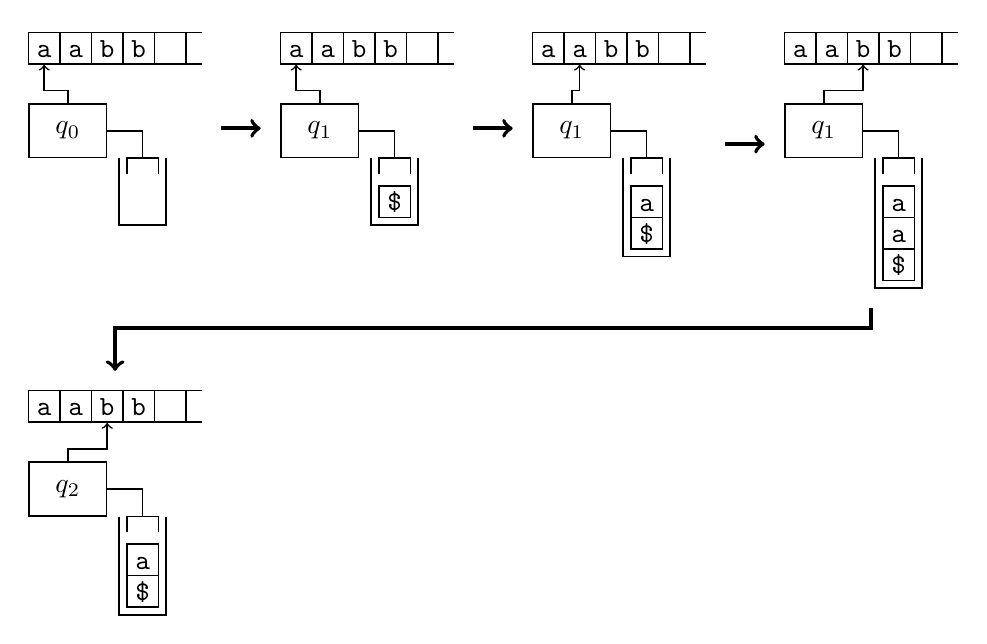
\begin{tikzpicture}

\draw (0.2, 0.2)
  node[draw, line width=0.02cm, , color=black,
       rounded corners=0cm, inner sep=0cm] {

\begin{minipage}[t][0.4cm]{0.4cm}
\mbox{}

\end{minipage}

};\draw (0.2, 0.2) node[color=black] {{\vphantom{aabb\SPACE}\texttt{a}}};
\draw (0.6000000000000001, 0.2)
  node[draw, line width=0.02cm, , color=black,
       rounded corners=0cm, inner sep=0cm] {

\begin{minipage}[t][0.4cm]{0.4cm}
\mbox{}

\end{minipage}

};\draw (0.6000000000000001, 0.2) node[color=black] {{\vphantom{aabb\SPACE}\texttt{a}}};
\draw (1.0, 0.2)
  node[draw, line width=0.02cm, , color=black,
       rounded corners=0cm, inner sep=0cm] {

\begin{minipage}[t][0.4cm]{0.4cm}
\mbox{}

\end{minipage}

};\draw (1.0, 0.2) node[color=black] {{\vphantom{aabb\SPACE}\texttt{b}}};
\draw (1.4000000000000001, 0.2)
  node[draw, line width=0.02cm, , color=black,
       rounded corners=0cm, inner sep=0cm] {

\begin{minipage}[t][0.4cm]{0.4cm}
\mbox{}

\end{minipage}

};\draw (1.4000000000000001, 0.2) node[color=black] {{\vphantom{aabb\SPACE}\texttt{b}}};
\draw (1.7999999999999998, 0.2)
  node[draw, line width=0.02cm, , color=black,
       rounded corners=0cm, inner sep=0cm] {

\begin{minipage}[t][0.4cm]{0.4cm}
\mbox{}

\end{minipage}

};\draw (1.7999999999999998, 0.2) node[color=black] {{\vphantom{aabb\SPACE}\texttt{\SPACE}}};\draw[line width=0.02cm,black] (2.0,0.4) to  (2.2,0.4);
\draw[line width=0.02cm,black] (2.0,0.0) to  (2.2,0.0);

\draw (0.5, -0.85)
  node[draw, line width=0.02cm, , color=black,
       rounded corners=0cm, inner sep=0cm] {

\begin{minipage}[t][0.68cm]{0.98cm}
\mbox{}

\end{minipage}

};\draw (0.5, -0.85) node[color=black] {$q_0$};\draw[line width=0.02cm,black,->] (0.5,-0.5) to  (0.5,-0.34) to  (0.2,-0.34) to  (0.2,-0.01);

\draw (1.45, -1.7499999999999998)
  node[draw=none, line width=0cm, , color=black,
       rounded corners=0cm, inner sep=0cm] {

\begin{minipage}[t][0.4cm]{0.4cm}
\mbox{}

\end{minipage}

};\draw[line width=0.02cm,black] (1.15,-1.2) to  (1.15,-2.05) to  (1.75,-2.05) to  (1.75,-1.2);
\draw[line width=0.02cm,black] (1,-0.85) to  (1.45,-0.85) to  (1.45,-1.2);
\draw[line width=0.02cm,black] (1.25,-1.4) to  (1.25,-1.2) to  (1.65,-1.2) to  (1.65,-1.4);
\draw[line width=0.05cm,black,->] (2.45,-0.82) to  (2.95,-0.82);

\draw (3.4000000000000004, 0.2)
  node[draw, line width=0.02cm, , color=black,
       rounded corners=0cm, inner sep=0cm] {

\begin{minipage}[t][0.4cm]{0.4cm}
\mbox{}

\end{minipage}

};\draw (3.4000000000000004, 0.2) node[color=black] {{\vphantom{\$aabb\SPACE}\texttt{a}}};
\draw (3.8, 0.2)
  node[draw, line width=0.02cm, , color=black,
       rounded corners=0cm, inner sep=0cm] {

\begin{minipage}[t][0.4cm]{0.4cm}
\mbox{}

\end{minipage}

};\draw (3.8, 0.2) node[color=black] {{\vphantom{\$aabb\SPACE}\texttt{a}}};
\draw (4.2, 0.2)
  node[draw, line width=0.02cm, , color=black,
       rounded corners=0cm, inner sep=0cm] {

\begin{minipage}[t][0.4cm]{0.4cm}
\mbox{}

\end{minipage}

};\draw (4.2, 0.2) node[color=black] {{\vphantom{\$aabb\SPACE}\texttt{b}}};
\draw (4.6000000000000005, 0.2)
  node[draw, line width=0.02cm, , color=black,
       rounded corners=0cm, inner sep=0cm] {

\begin{minipage}[t][0.4cm]{0.4cm}
\mbox{}

\end{minipage}

};\draw (4.6000000000000005, 0.2) node[color=black] {{\vphantom{\$aabb\SPACE}\texttt{b}}};
\draw (5.000000000000001, 0.2)
  node[draw, line width=0.02cm, , color=black,
       rounded corners=0cm, inner sep=0cm] {

\begin{minipage}[t][0.4cm]{0.4cm}
\mbox{}

\end{minipage}

};\draw (5.000000000000001, 0.2) node[color=black] {{\vphantom{\$aabb\SPACE}\texttt{\SPACE}}};\draw[line width=0.02cm,black] (5.200000000000001,0.4) to  (5.4,0.4);
\draw[line width=0.02cm,black] (5.200000000000001,0.0) to  (5.4,0.0);

\draw (3.7, -0.85)
  node[draw, line width=0.02cm, , color=black,
       rounded corners=0cm, inner sep=0cm] {

\begin{minipage}[t][0.68cm]{0.98cm}
\mbox{}

\end{minipage}

};\draw (3.7, -0.85) node[color=black] {$q_1$};\draw[line width=0.02cm,black,->] (3.7,-0.5) to  (3.7,-0.34) to  (3.4,-0.34) to  (3.4,-0.01);

\draw (4.65, -1.7499999999999998)
  node[draw, line width=0.02cm, , color=black,
       rounded corners=0cm, inner sep=0cm] {

\begin{minipage}[t][0.4cm]{0.4cm}
\mbox{}

\end{minipage}

};\draw (4.65, -1.7499999999999998) node[color=black] {{\vphantom{\$aabb\SPACE}\texttt{\$}}};\draw[line width=0.02cm,black] (4.35,-1.2) to  (4.35,-2.05) to  (4.95,-2.05) to  (4.95,-1.2);
\draw[line width=0.02cm,black] (4.2,-0.85) to  (4.65,-0.85) to  (4.65,-1.2);
\draw[line width=0.02cm,black] (4.45,-1.4) to  (4.45,-1.2) to  (4.85,-1.2) to  (4.85,-1.4);
\draw[line width=0.05cm,black,->] (5.65,-0.82) to  (6.15,-0.82);

\draw (6.600000000000001, 0.2)
  node[draw, line width=0.02cm, , color=black,
       rounded corners=0cm, inner sep=0cm] {

\begin{minipage}[t][0.4cm]{0.4cm}
\mbox{}

\end{minipage}

};\draw (6.600000000000001, 0.2) node[color=black] {{\vphantom{a\$aabb\SPACE}\texttt{a}}};
\draw (7.000000000000002, 0.2)
  node[draw, line width=0.02cm, , color=black,
       rounded corners=0cm, inner sep=0cm] {

\begin{minipage}[t][0.4cm]{0.4cm}
\mbox{}

\end{minipage}

};\draw (7.000000000000002, 0.2) node[color=black] {{\vphantom{a\$aabb\SPACE}\texttt{a}}};
\draw (7.400000000000002, 0.2)
  node[draw, line width=0.02cm, , color=black,
       rounded corners=0cm, inner sep=0cm] {

\begin{minipage}[t][0.4cm]{0.4cm}
\mbox{}

\end{minipage}

};\draw (7.400000000000002, 0.2) node[color=black] {{\vphantom{a\$aabb\SPACE}\texttt{b}}};
\draw (7.8000000000000025, 0.2)
  node[draw, line width=0.02cm, , color=black,
       rounded corners=0cm, inner sep=0cm] {

\begin{minipage}[t][0.4cm]{0.4cm}
\mbox{}

\end{minipage}

};\draw (7.8000000000000025, 0.2) node[color=black] {{\vphantom{a\$aabb\SPACE}\texttt{b}}};
\draw (8.200000000000003, 0.2)
  node[draw, line width=0.02cm, , color=black,
       rounded corners=0cm, inner sep=0cm] {

\begin{minipage}[t][0.4cm]{0.4cm}
\mbox{}

\end{minipage}

};\draw (8.200000000000003, 0.2) node[color=black] {{\vphantom{a\$aabb\SPACE}\texttt{\SPACE}}};\draw[line width=0.02cm,black] (8.400000000000002,0.4) to  (8.600000000000001,0.4);
\draw[line width=0.02cm,black] (8.400000000000002,0.0) to  (8.600000000000001,0.0);

\draw (6.900000000000001, -0.85)
  node[draw, line width=0.02cm, , color=black,
       rounded corners=0cm, inner sep=0cm] {

\begin{minipage}[t][0.68cm]{0.98cm}
\mbox{}

\end{minipage}

};\draw (6.900000000000001, -0.85) node[color=black] {$q_1$};\draw[line width=0.02cm,black,->] (6.9,-0.5) to  (6.9,-0.34) to  (7.0,-0.34) to  (7.0,-0.01);

\draw (7.850000000000001, -1.7499999999999998)
  node[draw, line width=0.02cm, , color=black,
       rounded corners=0cm, inner sep=0cm] {

\begin{minipage}[t][0.4cm]{0.4cm}
\mbox{}

\end{minipage}

};\draw (7.850000000000001, -1.7499999999999998) node[color=black] {{\vphantom{a\$aabb\SPACE}\texttt{a}}};
\draw (7.850000000000001, -2.1499999999999995)
  node[draw, line width=0.02cm, , color=black,
       rounded corners=0cm, inner sep=0cm] {

\begin{minipage}[t][0.4cm]{0.4cm}
\mbox{}

\end{minipage}

};\draw (7.850000000000001, -2.1499999999999995) node[color=black] {{\vphantom{a\$aabb\SPACE}\texttt{\$}}};\draw[line width=0.02cm,black] (7.55,-1.2) to  (7.55,-2.45) to  (8.15,-2.45) to  (8.15,-1.2);
\draw[line width=0.02cm,black] (7.4,-0.85) to  (7.85,-0.85) to  (7.85,-1.2);
\draw[line width=0.02cm,black] (7.65,-1.4) to  (7.65,-1.2) to  (8.05,-1.2) to  (8.05,-1.4);
\draw[line width=0.05cm,black,->] (8.85,-1.02) to  (9.35,-1.02);

\draw (9.8, 0.2)
  node[draw, line width=0.02cm, , color=black,
       rounded corners=0cm, inner sep=0cm] {

\begin{minipage}[t][0.4cm]{0.4cm}
\mbox{}

\end{minipage}

};\draw (9.8, 0.2) node[color=black] {{\vphantom{aa\$aabb\SPACE}\texttt{a}}};
\draw (10.200000000000003, 0.2)
  node[draw, line width=0.02cm, , color=black,
       rounded corners=0cm, inner sep=0cm] {

\begin{minipage}[t][0.4cm]{0.4cm}
\mbox{}

\end{minipage}

};\draw (10.200000000000003, 0.2) node[color=black] {{\vphantom{aa\$aabb\SPACE}\texttt{a}}};
\draw (10.600000000000001, 0.2)
  node[draw, line width=0.02cm, , color=black,
       rounded corners=0cm, inner sep=0cm] {

\begin{minipage}[t][0.4cm]{0.4cm}
\mbox{}

\end{minipage}

};\draw (10.600000000000001, 0.2) node[color=black] {{\vphantom{aa\$aabb\SPACE}\texttt{b}}};
\draw (11.000000000000004, 0.2)
  node[draw, line width=0.02cm, , color=black,
       rounded corners=0cm, inner sep=0cm] {

\begin{minipage}[t][0.4cm]{0.4cm}
\mbox{}

\end{minipage}

};\draw (11.000000000000004, 0.2) node[color=black] {{\vphantom{aa\$aabb\SPACE}\texttt{b}}};
\draw (11.400000000000002, 0.2)
  node[draw, line width=0.02cm, , color=black,
       rounded corners=0cm, inner sep=0cm] {

\begin{minipage}[t][0.4cm]{0.4cm}
\mbox{}

\end{minipage}

};\draw (11.400000000000002, 0.2) node[color=black] {{\vphantom{aa\$aabb\SPACE}\texttt{\SPACE}}};\draw[line width=0.02cm,black] (11.600000000000003,0.4) to  (11.800000000000002,0.4);
\draw[line width=0.02cm,black] (11.600000000000003,0.0) to  (11.800000000000002,0.0);

\draw (10.100000000000001, -0.85)
  node[draw, line width=0.02cm, , color=black,
       rounded corners=0cm, inner sep=0cm] {

\begin{minipage}[t][0.68cm]{0.98cm}
\mbox{}

\end{minipage}

};\draw (10.100000000000001, -0.85) node[color=black] {$q_1$};\draw[line width=0.02cm,black,->] (10.1,-0.5) to  (10.1,-0.34) to  (10.6,-0.34) to  (10.6,-0.01);

\draw (11.05, -1.7499999999999998)
  node[draw, line width=0.02cm, , color=black,
       rounded corners=0cm, inner sep=0cm] {

\begin{minipage}[t][0.4cm]{0.4cm}
\mbox{}

\end{minipage}

};\draw (11.05, -1.7499999999999998) node[color=black] {{\vphantom{aa\$aabb\SPACE}\texttt{a}}};
\draw (11.05, -2.1499999999999995)
  node[draw, line width=0.02cm, , color=black,
       rounded corners=0cm, inner sep=0cm] {

\begin{minipage}[t][0.4cm]{0.4cm}
\mbox{}

\end{minipage}

};\draw (11.05, -2.1499999999999995) node[color=black] {{\vphantom{aa\$aabb\SPACE}\texttt{a}}};
\draw (11.05, -2.55)
  node[draw, line width=0.02cm, , color=black,
       rounded corners=0cm, inner sep=0cm] {

\begin{minipage}[t][0.4cm]{0.4cm}
\mbox{}

\end{minipage}

};\draw (11.05, -2.55) node[color=black] {{\vphantom{aa\$aabb\SPACE}\texttt{\$}}};\draw[line width=0.02cm,black] (10.75,-1.2) to  (10.75,-2.85) to  (11.35,-2.85) to  (11.35,-1.2);
\draw[line width=0.02cm,black] (10.6,-0.85) to  (11.05,-0.85) to  (11.05,-1.2);
\draw[line width=0.02cm,black] (10.85,-1.4) to  (10.85,-1.2) to  (11.25,-1.2) to  (11.25,-1.4);
\draw[line width=0.05cm,black,->] (10.7,-3.1) to  (10.7,-3.35) to  (1.1,-3.35) to  (1.1,-3.9);

\draw (0.2, -4.35)
  node[draw, line width=0.02cm, , color=black,
       rounded corners=0cm, inner sep=0cm] {

\begin{minipage}[t][0.4cm]{0.4cm}
\mbox{}

\end{minipage}

};\draw (0.2, -4.35) node[color=black] {{\vphantom{a\$aabb\SPACE}\texttt{a}}};
\draw (0.6000000000000001, -4.35)
  node[draw, line width=0.02cm, , color=black,
       rounded corners=0cm, inner sep=0cm] {

\begin{minipage}[t][0.4cm]{0.4cm}
\mbox{}

\end{minipage}

};\draw (0.6000000000000001, -4.35) node[color=black] {{\vphantom{a\$aabb\SPACE}\texttt{a}}};
\draw (1.0, -4.35)
  node[draw, line width=0.02cm, , color=black,
       rounded corners=0cm, inner sep=0cm] {

\begin{minipage}[t][0.4cm]{0.4cm}
\mbox{}

\end{minipage}

};\draw (1.0, -4.35) node[color=black] {{\vphantom{a\$aabb\SPACE}\texttt{b}}};
\draw (1.4000000000000001, -4.35)
  node[draw, line width=0.02cm, , color=black,
       rounded corners=0cm, inner sep=0cm] {

\begin{minipage}[t][0.4cm]{0.4cm}
\mbox{}

\end{minipage}

};\draw (1.4000000000000001, -4.35) node[color=black] {{\vphantom{a\$aabb\SPACE}\texttt{b}}};
\draw (1.7999999999999998, -4.35)
  node[draw, line width=0.02cm, , color=black,
       rounded corners=0cm, inner sep=0cm] {

\begin{minipage}[t][0.4cm]{0.4cm}
\mbox{}

\end{minipage}

};\draw (1.7999999999999998, -4.35) node[color=black] {{\vphantom{a\$aabb\SPACE}\texttt{\SPACE}}};\draw[line width=0.02cm,black] (2.0,-4.1499999999999995) to  (2.2,-4.1499999999999995);
\draw[line width=0.02cm,black] (2.0,-4.55) to  (2.2,-4.55);

\draw (0.5, -5.4)
  node[draw, line width=0.02cm, , color=black,
       rounded corners=0cm, inner sep=0cm] {

\begin{minipage}[t][0.68cm]{0.98cm}
\mbox{}

\end{minipage}

};\draw (0.5, -5.4) node[color=black] {$q_2$};\draw[line width=0.02cm,black,->] (0.5,-5.05) to  (0.5,-4.89) to  (1.0,-4.89) to  (1.0,-4.56);

\draw (1.45, -6.300000000000001)
  node[draw, line width=0.02cm, , color=black,
       rounded corners=0cm, inner sep=0cm] {

\begin{minipage}[t][0.4cm]{0.4cm}
\mbox{}

\end{minipage}

};\draw (1.45, -6.300000000000001) node[color=black] {{\vphantom{a\$aabb\SPACE}\texttt{a}}};
\draw (1.45, -6.700000000000001)
  node[draw, line width=0.02cm, , color=black,
       rounded corners=0cm, inner sep=0cm] {

\begin{minipage}[t][0.4cm]{0.4cm}
\mbox{}

\end{minipage}

};\draw (1.45, -6.700000000000001) node[color=black] {{\vphantom{a\$aabb\SPACE}\texttt{\$}}};\draw[line width=0.02cm,black] (1.15,-5.75) to  (1.15,-7.0) to  (1.75,-7.0) to  (1.75,-5.75);
\draw[line width=0.02cm,black] (1,-5.4) to  (1.45,-5.4) to  (1.45,-5.75);
\draw[line width=0.02cm,black] (1.25,-5.95) to  (1.25,-5.75) to  (1.65,-5.75) to  (1.65,-5.95);
\end{tikzpicture}

\end{center}



the size is 3 and the capacity is 4.

Implement this type of linked list.
